\section{Considere el P.P.L.}
    \begin{tabular}{|l|l|}
    \hline
        Max & 8x_1+6x_2 \\ \hline
        ~ & x_1-x_2\leq \frac{3}{5} \\ \hline
        ~ & x_1-x_2\geq -2 \\ \hline
        ~ & x_1,x_2 \geq 0 \\ \hline
    \end{tabular}
    
    \begin{itemize}
        \item Resuelva los problemas primal y dual
        
        Tengamos que el problema primal es:
        
        \begin{tabular}{|l|l|}
    \hline
        Max & 8x_1+6x_2 \\ \hline
        ~ & x_1-x_2\leq \frac{3}{5}: w_1 \\ \hline
        ~ & x_1-x_2\geq -2: w_2 \\ \hline
        ~ & x_1,x_2 \geq 0 \\ \hline
    \end{tabular}
    
        Por metodo grafico tenemos:
        
        Podemos ver que la intersecci\'on de ambas restricciones no tiene ning\'un punto critico
        
        \centering
        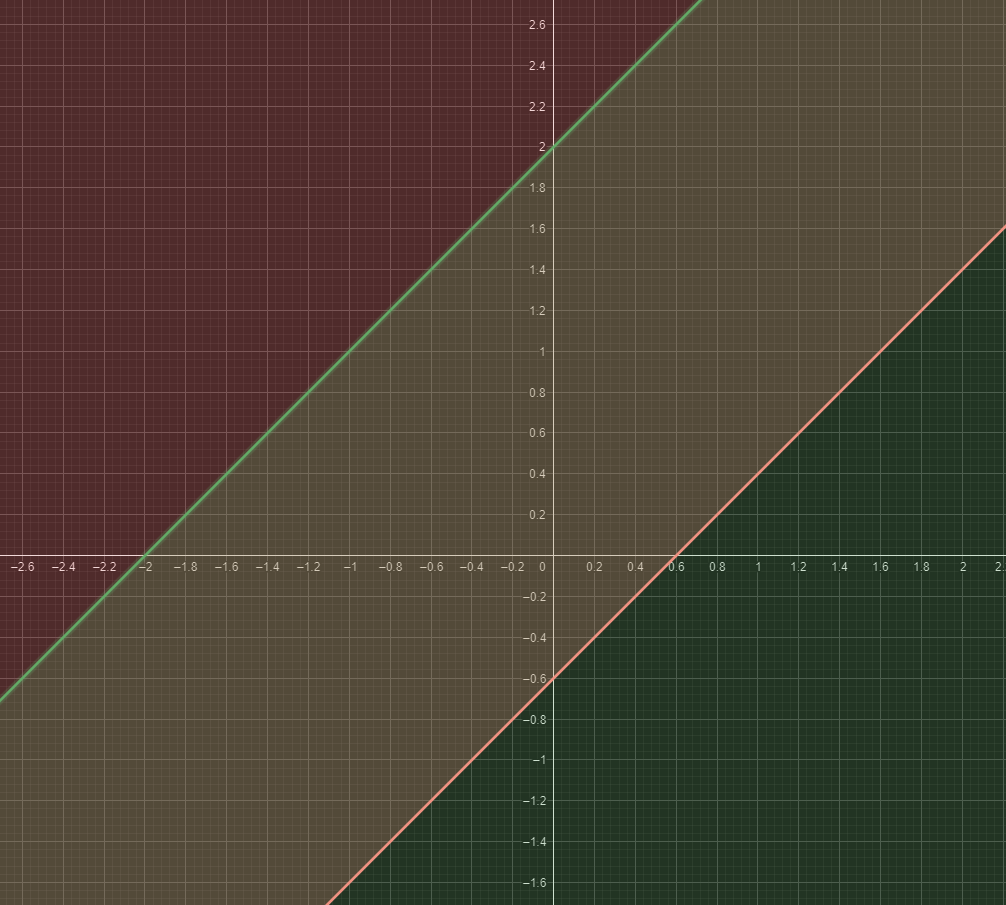
\includegraphics[scale=0.2]{Ejercicios/Imagenes/Ejercicio3a_1.png}\\
        Por lo que el problema no est\'a acotado y no existe una soluci\'on optima:
        
        \newpage
        
        Tengamos que el problema dual es:
        \begin{tabular}{|l|l|}
        \hline
        Min &  $z'=\frac{3}{2w_1}+2w_2$  \\ \hline
        ~ & w_1-w_2\geq 8 \\ \hline
        ~ & -w_1+w_2\geq 6 \\ \hline
        ~ & w_1,w_2 \geq 0 \\ \hline
        \end{tabular}
        Por el método gráfico tenemos:
        
        
        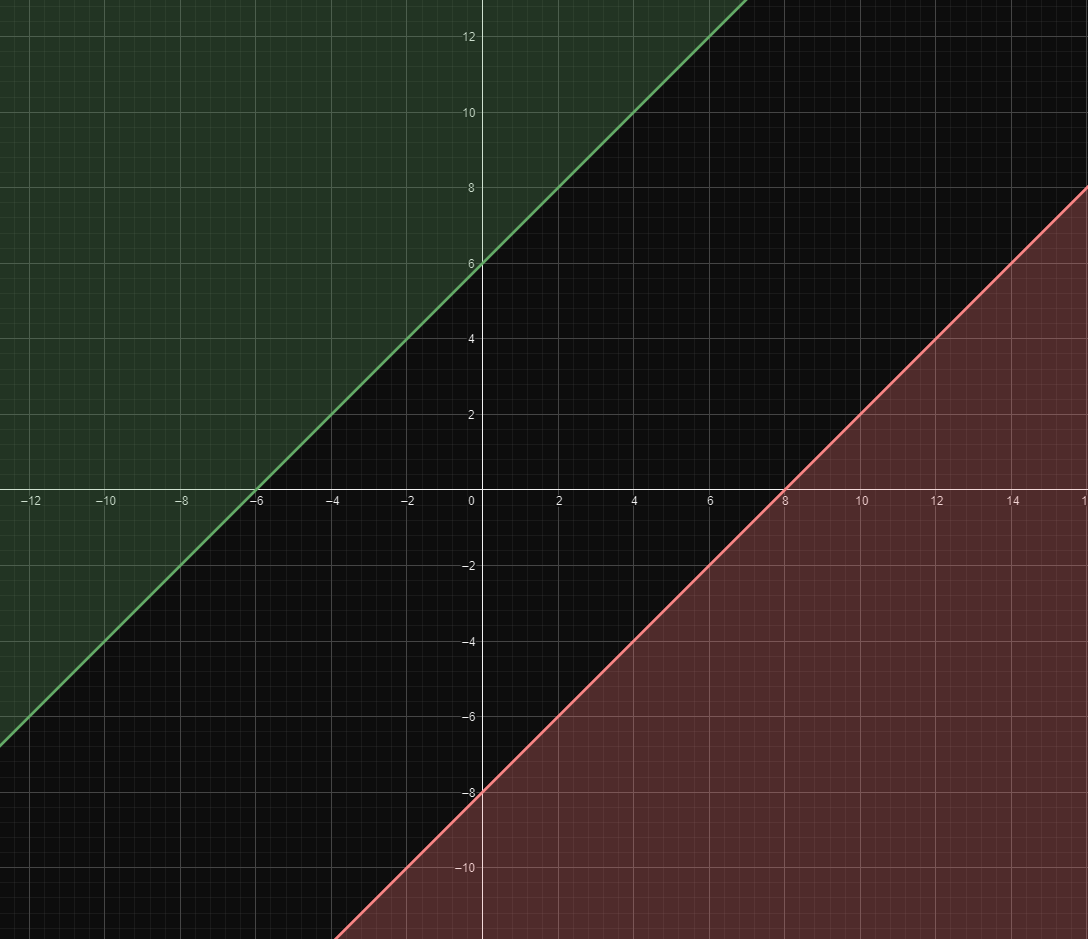
\includegraphics[scale=0.2]{Ejercicios/Imagenes/Ejercicio3a_2.png}
        
        Donde la intersección es vacia y por lo tanto no existe una solución factible
        
        \item Identifique el caso correspondiente en el Teorema de dualidad
    \end{itemize}